% !TEX root = lfgw.tex
\chapter{Präsentationen mit Beamer}
\autor{Axel Kielhorn}

\noindent Die Beamer Klasse bietet eine einfache Möglichkeit Präsentationen zu
erstellen.  Aufgrund der großen Auswahl an Themen und der reichhaltigen
Optionen, ist der Einstieg jedoch nicht so leicht.  Eine
Beispielpräsentation\footnote{%
\url{http://www.dante.de/events/dante2014/Programm/Vortraege/kielhorn-beamer.zip}}
zeigt einige Optionen und umschifft einige der Klippen, die sich einem 
Anfänger in den Weg stellen.

Mit Beamer lässt sich sowohl die Präsentation, als auch das Begleitmaterial
(Hand"-out) erstellen.  Dazu werden zwei Steuerdateien benötigt, eine für die
Präsentation, eine für den Ausdruck.

\section{Optionen -- Präsentation}

\begin{lfgwcode}{}
\documentclass[ignorenonframetext,%
utf8,
%aspectratio=169, % 16:9 (160 x 90 mm) default is 4:3 (128 x 96 mm)
%11pt, % 8pt, 9pt, 10pt, 11pt, 12pt, 14pt, 17pt
%draft,
%xcolor=dvipsnames, svgnames, x11names, 
]{beamer}
\end{lfgwcode}

Das Standardformat für die Ausgabe ist 128~mm $\times$ 96~mm, also im
Seitenverhältnis 4:3. Mit den Optionen \texttt{aspectratio=169} bzw.
\texttt{aspectratio=1610} lässt sich das Seitenverhältnis für
Breitbildprojektoren umschalten.  Zusätzlich gibt es noch die Formate
\texttt{149} (14:9), \texttt{141} (1,14:1; DIN A6), \texttt{32} (3:2;
Kleinbildfilm) und \texttt{54} (5:4).

Beamer nutzt \Package{xcolor} für die Farbdarstellung. Über die
entsprechenden Optionen können benannte Farben aus den entsprechenden
Farbräumen benutzt werden.

Über die Option \texttt{ignorenonframetext} wird sichergestellt, das für die
Präsentation nur der Inhalt der Frames berücksichtigt wird. Dies hat zur
Folge, das Anweisungen für die Präsentation explizit aktiviert werden
müssen.

Viele Beispiele im Internet gehen von einer reinen Präsentation aus, diese
müssen an geeigneten Stellen um ein

\begin{lfgwcode}{}
\mode<presentation>
{
...
}
\end{lfgwcode}

ergänzt werden.

\subsection{Das Aussehen der Präsentation: Themes}

Das Layout der Präsentation wird über sogenannte Themes gesteuert. Ohne
Angabe wird das \texttt{default} Theme verwendet. Unter
\url{http://www.hartwork.org/beamer-theme-matrix/} gibt es eine Liste mit
allen Themes, kombiniert mit allen Farb-Themes.

\begin{lfgwcode}{}
\mode<presentation>
{
  %\usetheme{CambridgeUS}        % rot
  %\usetheme{EastLansing}        % grün einfach
  %\usetheme{Copenhagen}         % blau mit section / subsection im Kopf
  %\usetheme{Montpellier}        % blau mit Navigationsbaum im Kopf 
  %\usetheme{Antibes}            % blau mit Navigationsbaum im Kopf
  %\usetheme{JuanLesPins}        % blau mit Navigationsbaum im Kopf mit Schatten
  %\usetheme{Ilmenau}            % blau mit Fortschrittsanzeige
  %\usetheme{Bergen}             % blau mit Seitenleiste
  %  \def\insertauthorindicator{Wer\,?}         % Who
  %  \def\insertinstituteindicator{Vom\,?}      % From
  %  \def\insertdateindicator{Wo\,?}            % When
  %  \setbeamercolor{description item}%
  %    {use=structure,bg=white,fg=structure.fg!75!black}
  %  \setbeamercolor{description item}%
  %    {use=structure,bg=white,fg=structure.fg}
  %\usetheme[width=20mm]{Berkeley} % blau mit Inhaltsverzeichnis
  \usetheme[width=20mm]{PaloAlto} % blau mit Inhaltsverzeichnis abgerundet
  %\usetheme{PaloAlto} % blau mit Inhaltsverzeichnis abgerundet
  %\usetheme[width=20mm]{Hannover} % hellblau mit Inhaltsverzeichnis
  %
  %\pgfdeclareimage[width=16mm]{logo}{DANTE2klein}
  %\logo{\pgfuseimage{logo}}
}
\end{lfgwcode}

Bei Themes der \texttt{Berkeley} Klasse (farbiger Streifen am linken Rand)
lässt sich die Breite des Streifens über eine Option einstellen.

Das Theme \texttt{Bergen} benutzt einige fest kodierte Texte, diese müssen
bei Bedarf angepasst werden.  Außerdem erzeugt es bei \texttt{description}
Umgebungen weißen Text auf weißem Grund.

Das Logo wird an einer von Theme vorgegebenen Stelle eingefügt, der Anwender
hat darauf keinen Einfluss.

\subsection{Farbe -- mehr oder weniger}

Über ein Farb-Thema (Colortheme) lässt sich die Farbe der Präsentation
einstellen.  Bei den grauen Farb-Themen sind einige Hervorhebungen
(\texttt{example} Umgebung) nicht hervorgehoben.  Diese müssen bei Bedarf
angepasst werden.

\begin{lfgwcode}{}
\mode<presentation>
  %\usecolortheme{spruce}                    % grün
  %\usecolortheme[named=MSUgreen]{structure} % für Aufzählungen
  %\usecolortheme{albatross}                 % blau bunt
  %\usecolortheme[overlystylish]{albatross}  % blau bunt
  %\usecolortheme{beetle}                    % blau grau
  %\usecolortheme{crane}                     % gelb orange
  %\usecolortheme{dove}                      % grau
  \usecolortheme{seagull}                    % grauer
}
\end{lfgwcode}

\subsection{Globale Einstellungen}

Eine häufig benutzte Option von Beamer ist das stückweise (inkrementelle)
Aufdecken.  Dies kann global für alle Umgebungen die dies unterstützen
eingeschaltet werden. Sollten einzelne komplett angezeigt werden, so kann
die globale Einstellung durch Angabe von \texttt{<*>} bei den entsprechenden
Befehlen überschrieben werden.

Außerdem ist es möglich, den noch nicht angezeigten
Text transparent darzustellen.

Am rechten unteren Rand erscheinen Navigationssymbole, diese lassen sich
konfigurieren oder ganz ausschalten.

\begin{lfgwcode}{}
\mode<presentation>
{
% Falls Aufzählungen immer schrittweise gezeigt werden sollen, 
% kann folgendes Kommando benutzt werden:
  \beamerdefaultoverlayspecification{<+->}
% Aufzählungen mit Vorschau zeigen
  \setbeamercovered{transparent}
% Navigationssymbole
  %\setbeamertemplate{navigation symbols}[default]  % horizontal
  %\setbeamertemplate{navigation symbols}[vertical] % vertikal
  %\setbeamertemplate{navigation symbols}[only frame symbol]
  \setbeamertemplate{navigation symbols}{}          % keine
}
\end{lfgwcode}

\subsection{Teilweise Bearbeitung}

Bei Umfangreichen Präsentationen kann es sinnvoll sein, nur den aktuellen
Frame zu bearbeiten.  Mit \cs{includeonlyframes} kann man die zu
bearbeitenden Frames festlegen.  Wenn der aktuelle Frame den
\texttt{label=current} trägt, so wird nur dieser Frame bearbeitet.  Ist die
Bearbeitung abgeschlossen, wird der Label entfernt und im nächsten Frame
gesetzt.  Zur Bearbeitung des kompletten Dokuments wird die Zeile
auskommentiert.

Wird ein Label mehrfach verwendet, gibt es eine Warnung in der
\texttt{.log}-Datei, das Dokument wird aber trotzdem komplett bearbeitet.

\begin{lfgwcode}{}
\includeonlyframes{current}
\end{lfgwcode}

Zum Schluss wird die eigentliche Präsentation geladen:

\begin{lfgwcode}{}
\input{Beamerws}
\end{lfgwcode}

\section{Optionen -- Article}

Die Steuerdatei für die Papierversion ist deutlich einfacher. Es wird
lediglich die Dokumentklasse und das Paket \Package{beamerarticle} geladen.

Beamer befindet sich jetzt im \textit{Article} Modus. 

Bei der Bearbeitung wird auch der Text zwischen den Frames berücksichtigt.

\begin{lfgwcode}{}
\documentclass[a4paper,11pt]{article}
\usepackage{beamerarticle}
\input{Beamerlfgw}
\end{lfgwcode}

\section{Die Präsentation}

\subsection{Präambel}

Alle gemeinsamen Einstellungen sollten im Hauptdokument vorgenommen werden.
Bei den Schriften ist darauf zu achten, das Beamer die serifenlose Schrift benutzt.
Einige Schriften sind nicht vorhanden wenn man die \texttt{small} Version von 
\TeXLive{} installiert.

\begin{lfgwcode}{}
\usepackage[utf8]{inputenc}
\usepackage[german]{babel}
%
% Schriften
%
\usepackage[TS1,T1]{fontenc}
%\usepackage{charter}   \renewcommand{\sfdefault}{bch}
%\usepackage{utopia}    \renewcommand{\sfdefault}{put}
%\usepackage{lmodern}
\usepackage{dejavu}
%\usepackage{PTSans}
\end{lfgwcode}

Angaben für die Titelseite, eine Kurzform in eckigen Klammern ist möglich.

\begin{lfgwcode}{}
\title{Präsentationen mit Beamer}
%\subtitle {Untertitel} % (optional)
\author{Axel Kielhorn}
\date[LFGW]{Präsentation zum Buch}
\end{lfgwcode}

\subsection{Der Inhalt}

\begin{lfgwcode}{}
\begin{document}
\end{lfgwcode}

Eine Beamer Präsentation besteht aus Rahmen (Frames).
Ist die Option \texttt{ignorenonframetext} gesetzt, wird alles außerhalb
eines Frames für die Präsentation ignoriert. Eine Ausnahme bilden hier 
die Gliederungsbefehle \cs{section}, \dots.

Es gibt zwei Möglichkeiten einen Frame zu definieren.
Die \LaTeX\ Methode und die \TeX\ Methode. Bei letzterer muss der
\cs{frametitle} über einen Befehl eingegeben werden, bei der ersten ist
auch ein optionales Argument möglich. 

\subsection{Rahmen}
\begin{lfgwcode}{}
\begin{frame}{Rahmen}
    Inhalt
\end{frame}

\frame{
      \frametitle{Rahmen}
      Inhalt
      }
\end{lfgwcode}

\subsection{Overlayspezifikationen}

Beamer erzeugt aus einem Frame eine oder mehrere PDF-Seiten.
Welcher Frame-Inhalt auf welcher Seite erscheint, bestimmt die
Overlayspezifikation. Diese kann für den gesamten Frame oder Teile davon
gelten.

Die Overlayspezifikation wird in spitzen Klammern in \cs{frame}-Befehl 
angegeben, in diesem Fall gilt sie für den gesamten Frame.
Die Overlayspezifikation \texttt{<beamer>} bewirkt, das dieser Frame nur im Modus
\textit{Beamer} erscheint, im Modus \textit{Article} wird er unterdrückt.

Die Overlayspezifikation \texttt{[<*>]} sorgt für komplettes Aufdecken, auch
wenn für das Dokument inkrementelles Aufdecken definiert ist. (Wirkt sich
nur für \texttt{Bergen} aus.) 

Die Papierversion erhält ebenfalls eine Titelseite, da der Befehl außerhalb
eines Frames steht, wird er in der Präsentation ignoriert.

\begin{lfgwcode}{}
\begin{frame}<beamer>[<*>][label=titel]{}
  \titlepage
\end{frame}

\maketitle % Für article
\end{lfgwcode}

Das Inhaltsverzeichnis erscheint ebenfalls nur in der Präsentation.

\begin{lfgwcode}{}
\begin{frame}<beamer>{Inhalt}
% Nur im Beamer-Mode anzeigen 
   \tabelofcontents[pausesections]
\end{frame}
\end{lfgwcode}

Die Option \texttt{pausesections} führt zu einer inkrementellen Ausgabe, bei
der für jede Section eine neue Seite erzeugt wird. Alternativ kann man auch
\texttt{currentsection} angeben, dann werden nur die vorherige und die aktuelle Section
angezeigt, die vorherige Section erscheint transparent.

Möchte man nur die Sections ohne Subsections aufführen, 
so lassen sich letztere mit der Option \texttt{hideallsubsections} unterdrücken.

\begin{lfgwcode}{}
    \tableofcontents[currentsection] % nur aktuelle Section
\end{lfgwcode}

\subsection{Inkrementelle Aufzählungen}

Sehr beliebt sind die nacheinander aufgedeckten Aufzählungspunkte.
Sie werden durch die Overlayspezifikation \texttt{<+->} 
aktiviert und erzeugen für jeden Aufzählungspunkt eine neue Seite.

\begin{lfgwcode}{}
\begin{itemize}[<+->]
  \item Erstens
  \item Zweitens
  \item Drittens
\end{itemize}
\end{lfgwcode}

Möchte man mehr Kontrolle, so gibt es die Möglichkeit die
Overlayspezifikationen direkt anzugeben. Im folgenden Beispiel werden die
beiden letzten Punkte gleichzeitig aufgedeckt.

\begin{lfgwcode}{}
\begin{itemize}
  \item <1->Erstens
  \item <2->Zweitens
  \item <3->Drittens
  \item <3->"`Drittens"' in einer postsekundaren Gesellschaft
\end{itemize}
\end{lfgwcode}

Gleiches lässt sich auch mit weniger Schreibarbeit erreichen, indem man als
Spezifikation \texttt{<.->} angibt.

\begin{lfgwcode}{}
\begin{itemize}[<+->]
  \item Erstens
  \item Zweitens
  \item Drittens
  \item <.->"`Drittens"' in einer postsekundaren Gesellschaft
\end{itemize}
\end{lfgwcode}

Eine weiter Möglichkeit Overlayspezifikationen einzusetzen bietet der
\cs{only} Befehl. Mit ihm lässt sich in einem Frame Text ausgeben, der
nur in der \textit{Article} Version erscheint.

\begin{lfgwcode}{}
\begin{itemize}[<+->]
  \item Erstens
    \only<article>{Erklärung zu Erstens, nur im \textit{Article}.}
  \item Zweitens
    \only<article>{Erklärung zu Zweitens.}
  \item Drittens
    \only<article>{Erklärung zu Drittens.}
\end{itemize}
\end{lfgwcode}

Bei \texttt{description} Umgebungen kann es leicht passieren, das der
Aufzählungstext nicht in den reservierten Bereich passt. Das führt dann zu
einer hässlichen Aufzählung, wie in Abbildung~\ref{fig:aufz1} zu sehen ist.

\begin{lfgwcode}{}
\begin{description}[<*>]
  \item[Spruce]
    Dezent
  \item[Pointless Albatross]
    Aufdringlich
  \item[Beetle]
    Seriös
\end{description}
\end{lfgwcode}

\begin{figure}
  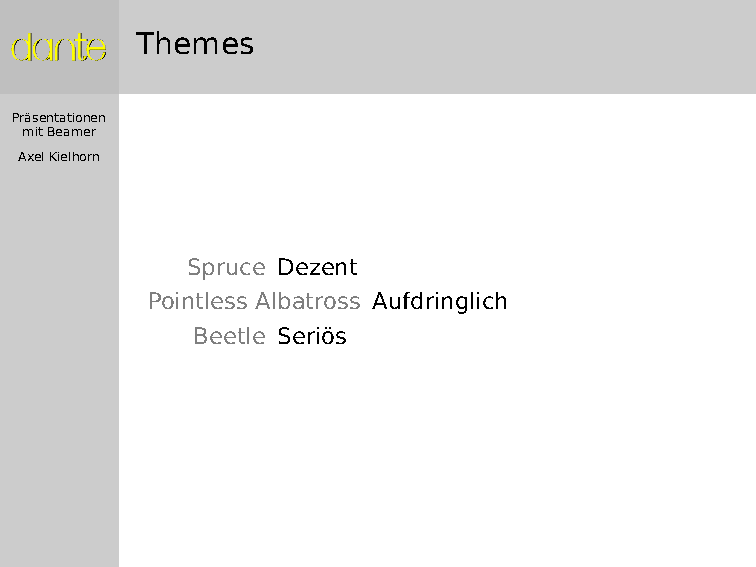
\includegraphics[width=\textwidth]{beamer-aufz1}
  \caption{Eine unschöne \texttt{description}.}
  \label{fig:aufz1}
\end{figure}

Mit einem optionalen Argument lässt sich das jedoch leicht beheben. (Abbildung~\ref{fig:aufz2})

\begin{lfgwcode}{}
\begin{description}[<*>][Pointless Albatross]
  \item[Spruce]
    Dezent
  \item[Pointless Albatross]
    Aufdringlich
  \item[Beetle]
    Seriös
\end{description}
\end{lfgwcode}

\begin{figure}
  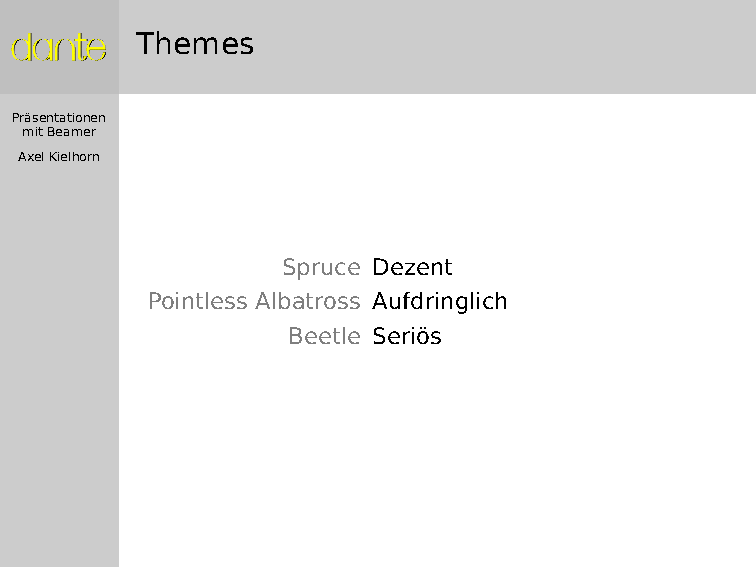
\includegraphics[width=\textwidth]{beamer-aufz2}
  \caption{Mit wenig Aufwand repariert.}
  \label{fig:aufz2}
\end{figure}

Auffälliger als Aufzählungen sind Blöcke. Beamer stellt drei Versionen zur
Verfügung, neben dem normalen \texttt{block} gibt es den \texttt{alertblock}
in rot und den \texttt{exampleblock} in grün. Da die Farben in einem grauen 
Farbtheme nicht erkennbar sind, wurde für Abbildung~\ref{fig:block} die 
Schrift verändert.

\begin{lfgwcode}{}
\setbeamerfont{block title example}{shape=\itshape}
\setbeamerfont{block body example}{family=\ttfamily}
\end{lfgwcode}

\begin{lfgwcode}{}
\begin{block}{Erstens}
    Nicht vergessen!
\end{block}
\begin{alertblock}{Zweitens}
    Unbedingt dran denken!
\end{alertblock}
\begin{exampleblock}{Drittens}
    Sehr wichtig!
\end{exampleblock}
\end{lfgwcode}

\begin{figure}
  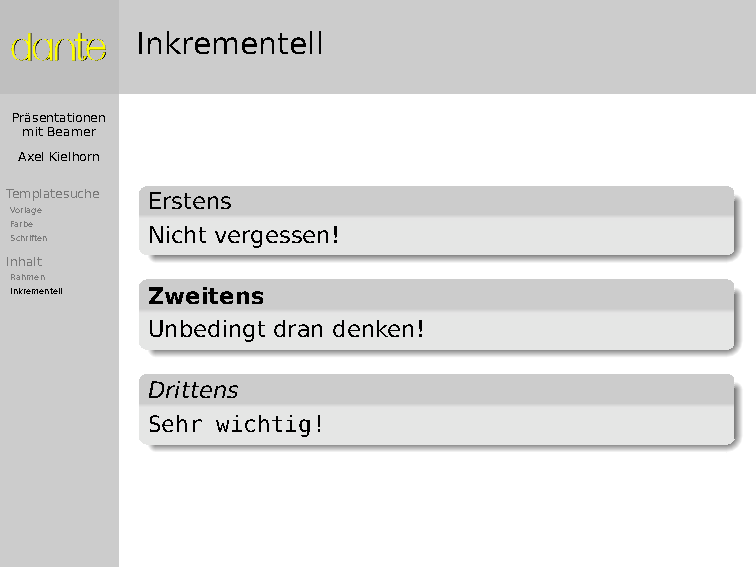
\includegraphics[width=\textwidth]{beamer-block}
  \caption{Blöcke statt Aufzählungen}
  \label{fig:block}
\end{figure}

\subsection{Inkrementelle Tabellen}

Bei Tabellen ist der Aufwand deutlich größer, es muss jedem Objekt
mitgeteilt werden, wann es sichtbar sein soll. Dies geschieht mit dem
\cs{uncover}-Befehl. Die Overlayspezifikationen \texttt{<2>} gibt an, das das
Objekt nur auf Seite 2 sichtbar ist. 

\begin{lfgwcode}{}
\begin{tabular}{llrrr}
Version    & Wert 1 & Wert 2          & \uncover<2>{Wert 2} \\
           &        &                 & \uncover<2>{optimiert}\\
2.7        & $0.85$ &           39\%  & \uncover<2>{35\%}\\
2.8        & $0.95$ & \alert<2>{49\%} & \uncover<2>{\alert<2>{44\%}}\\
2.9        & $0.98$ &           55\%  & \uncover<2>{51\%}
\end{tabular}
\end{lfgwcode}

Mehrere Objekte lassen sich in der \texttt{columns} Umgebung nebeneinander
platzieren. Die Spalten können oben \texttt{[t]}, unten \texttt{[b]} oder
zentriert \texttt{[c]} ausgerichtet werden.

Diese Art des Mehrspaltensatzes funktioniert nicht im
\textit{Article} Modus.

\begin{lfgwcode}{}
\begin{columns}[t]
  \begin{column}<1->{0.5\textwidth}
    Es ist so eng hier. Muss man das denn unbedingt zweispaltig setzen?
  \end{column}%
  \begin{column}<2->{0.5\textwidth}
    Ich will raus!
  \end{column}
\end{columns}
\end{lfgwcode}
  
\subsection{Übergänge}

Beamer unterstützt animierte Seitenwechsel, jedoch nur bei Verwendung von
Acrobat Reader, Evince oder Okular im Vollbildmodus. Die Befehle müssen auf
der Zielseite gegeben werden und gelten beim blättern auf diese Seite. Werden
sie für einen Frame gegeben, gelten sie für alle Seiten des Frames.

\begin{labeling}{\texttt{transblindshorizontal}}
  \item[\texttt{transdissolve}] Eine Seite löst sich in Punkten auf und eine neue entsteht
  \item[\texttt{transblindshorizontal}] oder \texttt{vertical}, der Jalousie-Effekt.
  \item[\texttt{transboxin}] oder \texttt{boxout}, rein- oder rauszoomen.
  \item[\texttt{transwipe}] Neue Seite wischt alte Seite weg.
\end{labeling}

\subsection{Sprünge}

Frames mit einem \texttt{label} können als Sprungziele verwendet werden.
Außerdem ist es möglich explizite Sprungziele zu definieren. Über einen
Hyperlink können diese Ziele angesprungen werden. Bei den Buttons handelt es
sich nur um Bilder, der \cs{beamerreturnbutton} bietet keine
Zurück-Funktion im Sinne eines Sprung-Stacks.

\begin{lfgwcode}{}
\hypertarget{Bilder}{}
\hyperlink{Bilder}{\beamergotobutton{Zu Bilder springen}}
\hyperlink{Bilder}{\beamerskipbutton{Zu Bilder springen}}
\hyperlink{Bilder}{\beamerreturnbutton{Zurück zu Bilder}}
\end{lfgwcode}

\begin{figure}
  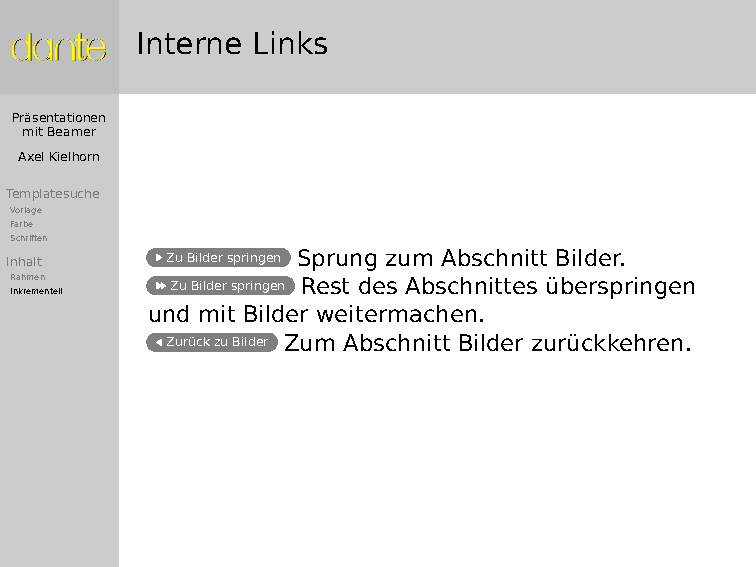
\includegraphics[width=\textwidth]{beamer-sprung}
  \caption{Sprünge zur näheren Erläuterung, oder bei Zeitmangel.}
  \label{fig:sprung}
\end{figure}

Die Überschriften im linken Rand sind ebenfalls Links.
Hier kann man schnell zum gewünschten Abschnitt springen.

\subsection{Bilder}

Bilder lassen sich wie gewohnt mit \cs{includegraphics} einbinden.

\begin{lfgwcode}{}
\includegraphics[width=\textwidth]{Bild.png}
\end{lfgwcode}

Benötigt man für ein großes Bild besonders viel Platz, kann man einen
\texttt{plain} Frame erzeugen. In diesem Fall ist die unterschiedliche
Skalierung für \textit{Beamer} und \textit{Article} zu beachten.

\begin{lfgwcode}{}
\begin{frame}[plain]
  \begin{centering}%
    \pgfimage<beamer>[width=1\paperwidth]{Bild.png}%
    \pgfimage<article>[width=1\textwidth]{Bild.png}%
    \par%
  \end{centering}%
\end{frame}
\end{lfgwcode}

Bei Themes mit farbigen Balken an der linken Seite funktioniert das nicht.
Hier muss für den \texttt{plain} Rahmen etwas mehr Aufwand getrieben werden.
Außerdem sind zwei \TeX-Läufe erforderlich.

\begin{lfgwcode}{}
\begin{frame}<beamer>[plain]
   \begin{tikzpicture}[remember picture,overlay]
      \node[at=(current page.center)] {\pgfimage[width=1\paperwidth]
      {Bild.png}};
   \end{tikzpicture}
\end{frame}
\end{lfgwcode}

\subsection{Tikz im Beamer}

Overlayspezifikationen funktionieren nicht nur für Text.
Im folgenden Beispiel wird im ersten Durchlauf das Koordinatenkreuz
gezeichnet und auf der zweiten Seite die Funktion geplottet.

Damit die zweite Seite nicht durchscheint und das Ergebnis verrät wird der
Uncovermodus explizit auf \texttt{invisible} gesetzt.

\begin{lfgwcode}{}
\mode<presentation>{
  \setbeamercovered{invisible}
}

\begin{frame}[fragile,label=tikz]{Tikz}
  \begin{tikzpicture}[scale=0.6]
     \draw[help lines] (0,0) grid (13,4);
     \draw[gray] (-0.4,0) node {0} (-0.4,1) node {1} 
                 (-0.4,2) node {2} (-0.4,3) node {3} (-0.4,4) node {4};
     \draw[gray] (0,-.4)  node {0} (3,-.4)  node {3} 
                 (6,-.4)  node {6} (9,-.4)  node {9} (12,-.4) node {12};
      \pgfplothandlerlineto 
      \onslide<2>\pgfplotxyfile{Daten.dat}
      \pgfusepath{stroke}
  \end{tikzpicture}
\end{frame}
\end{lfgwcode}

\subsection{Hintergrundbilder}

Natürlich kann man den Standardhintergrund durch ein Bild ersätzen, entweder
für die gesamte Präsentation, oder für einzelne Frames. Auch hier ist es
erforderlich den Präsentationsmodus zu aktivieren, um das
\texttt{backgroundtemplate} zu definieren.

\begin{lfgwcode}{}
\mode<presentation>{
\usebackgroundtemplate{\includegraphics[width=\paperwidth]{Hintergrund}}
}

\begin{frame}<beamer>[plain,b] % b = bottom
  \huge\bfseries\color{structure!15} Noch Fragen?
  \vspace{0.3cm} % Etwas Luft nach unten
\end{frame}

\mode<presentation>{
\usebackgroundtemplate{}
}
\end{lfgwcode}

Und damit schließt die Präsentation.

\begin{lfgwcode}{}
\end{document}
\end{lfgwcode}


\begin{thebibliography}{10}
      
  \bibitem{Tantau-Beamer} Till Tantau, Joseph Wright, Vedran Miletić.                    
      \newblock \emph{The beamer class}.                                        

  \bibitem{Voss-PML} Herbert Voß.              
      \newblock \emph{Präsentationen mit LaTeX}.                                        

\end{thebibliography}

beamer\footcite{voss:praesentationen}


